\chapter{Data Analysis and Machine Learning}
This chapter will discuss the steps that were followed during the analysis of the collected data. First we should look into the intermediary analysis that was conducted while data was being collected. Then the different data preprocessing steps will be justified and explained. Thirdly, we will present the results and motivation of a clustering attempt on the previously constructed vectors. And finally we will dive into the main matter of failure prediction models. 

\section{Intermediary Analysis}
Data collection required some time before it would produce a relevant dataset. With, on average, 112 failing CPEs\footnote{according to our ground truth} every day we would need some time in order to obtain a balanced dataset of sufficient size.

We leveraged this period of time in order to perform some initial analysis. We were interested in two main topics, first we wanted to determine how much did weekends influence the distribution of vectors, secondly we were interested in an exploratory data analysis that would give us a better understanding of the dataset. 

\subsection{Influence of Weekends on Vectors} 
\label{subsec:influence}
Choices that we did during the dataset's construction frequently needed to be arbitrary, even though they were motivated by network experts. Nevertheless, one of our main concerns was around data seasonality. 

Hopefully some of the seasonality is already being taken care of but there are many sources of such:
\begin{itemize}[topsep=0pt]
	\item \textbf{Over hours of the day}: because all vectors are constructed over the exact same hours, we are confident that they are comparable with respect to such seasonality. 
	\item \textbf{Over period of the year}: according to the HFC support expert, the temperature, as an example, could influence the performance of the network and the range of 'standard' values. Nevertheless, due to evident time restriction this couldn't be evaluated. We could argue that this  effect could be attenuated by considering a training dataset constructed on a limited number of past days to train on period specific patterns. 
	\item \textbf{Over days of week}: metrics of the network are highly dependent on the utilisation of each CPE, this is why we surmise a potential influence of the fact that Day\textsubscript{0} is or not a weekend day.
\end{itemize}

We decided to study the latter as we had the data that could help us get a feeling for such problem. An initial naïve analysis based on single variable hypothesis testing was performed to determine whether each feature displayed some evidence of different sampling distribution using the weekend and weekday populations. Then a more refined test based on bootstrapped energy statistics~\cite{energy_test} was implemented. 

We focused on the vectors composed of Day\textsubscript{0} 6-hour window averaged in relative format\footnote{We only consider the past 24 hours and discard the other days}.

\subsubsection{Naïve Approach: Kolmogorov-Smirnov statistic on 2 samples}
The Kolmogorov-Smirnov (KS) test~\cite{wiki:ks_test} is one of the most standard approaches to perform such test. It allows to test whether two populations are likely to be drawn from two distinct sampling distributions. The test isn't so meaningful in our case given that we are in a multivariate case with our vectors. Nevertheless it offers some interesting initial approach as we could observe features that show the most evidence of different sampling distributions.

We should first define the statistical terms that will be used in the following discussion:
\begin{itemize}[noitemsep,topsep=0pt]
	\item \textbf{Null Hypothesis}~\cite{wiki:null_hyp} ($H_0$): is the hypothesis that the test is trying to reject. Here: the two variables come from identical distributions.
	\item \textbf{Test statistic} ($T$): computed from the data and chosen such that large values of $T$ provide evidence against $H_0$. The observed value of $T$, $t_\text{obs}$ is compared to the distribution of $T$ under the null hypothesis. 
	\item \textbf{Significance level} (e.g. $\alpha = 0.05$): represents the probability of rejecting the null hypothesis when it is true. 
	\item \textbf{Confidence level}: indicating how sure you are of your decision to reject the null hypothesis given the observed test statistic ($CL = (1 -\alpha)\times 100\%$).
	\item \textbf{P-value}~\cite{wiki:pvalue}: $p=P_0(T \ge t_\text{obs})$, where $P_0$ is the probability under the null distribution. \textbf{Low values of $p$ suggest that the null hypothesis is false.} If the p-value is under the significance level, we can reject the null hypothesis for the given confidence level.
\end{itemize}

The KS test can be used either by comparing a given variable to a known distribution or directly by comparing two variables which is how we will use it here as we do not have information regarding the underlying distribution of features. 

The test was initially performed on each feature of the feature space which wasn't correct. Indeed, it is designed to be used on continuous distributions. Many features are discrete as for example the \texttt{MISS\_*}. 

Running the test on all continuous features, we focused our attention on features that yielded the lowest p-value as this should be the features for which we are the most confident on rejecting the null hypothesis. 

\begin{table}[h]
\begin{center}
\begin{tabular}{c r r}
\hline
\textbf{Feature} & \textbf{$t_\text{obs}$} & $p$\\ 
\hline\hline
\texttt{CER\_UP\_12H} & $0.128066$ &	 $2.547019\times 10^{-198}$\\
\hline
\texttt{CER\_UP\_6H} &  $0.094043$ & $3.869613\times 10^{-107}$\\
\hline
\texttt{CER\_DN\_18H} & $0.092828$ &	 $2.120185\times 10^{-104}$\\
\end{tabular}
\end{center}
\caption{\label{CPEMes}Features at the CPE level}
\end{table}

\begin{figure}[ht]
    \begin{center}
    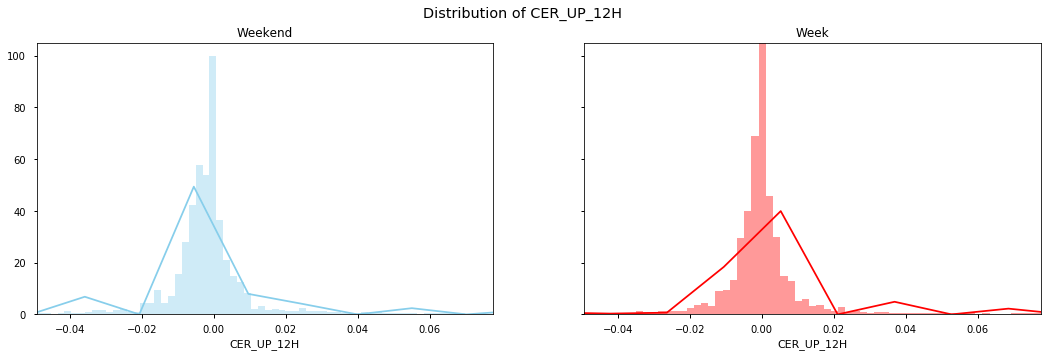
\includegraphics[width=1\linewidth]{images/KS_CER_UP_12.png}    
    \end{center}
    \caption{Comparison of distributions between the weekend and weekday population for \texttt{CER\_UP\_12H}}
    \label{KS_CER_UP_12}
\end{figure}

\begin{figure}[ht]
    \begin{center}
    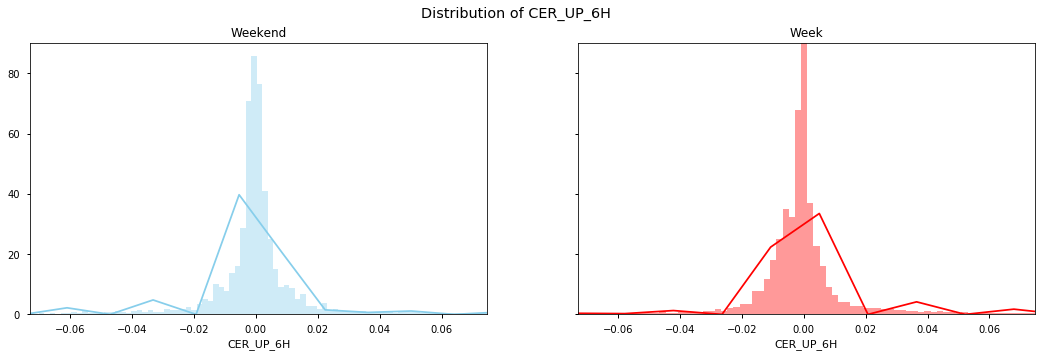
\includegraphics[width=1\linewidth]{images/KS_CER_UP_6.png}    
    \end{center}
    \caption{Comparison of distributions between the weekend and weekday population for \texttt{CER\_UP\_6H}}
    \label{KS_CER_UP_6}
\end{figure}

\begin{figure}[ht]
    \begin{center}
    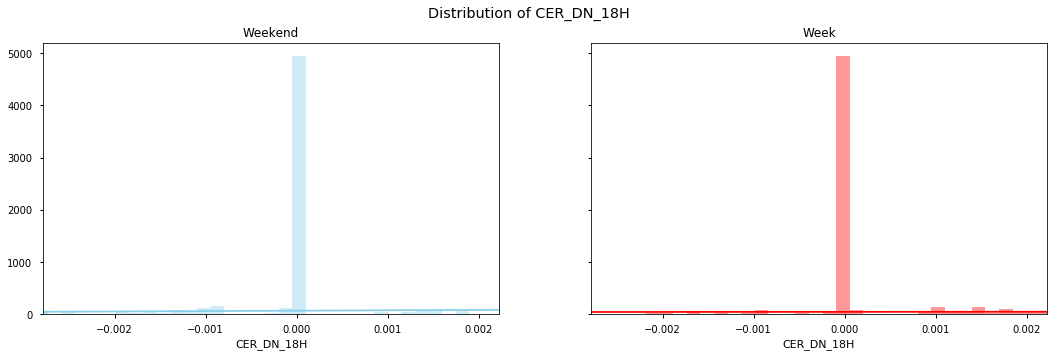
\includegraphics[width=1\linewidth]{images/KS_CER_DN_18.png}    
    \end{center}
	\caption{Comparison of distributions between the weekend and weekday population for \texttt{CER\_DN\_18H}}
    \label{KS_CER_DN_18}
\end{figure}

\begin{figure}[ht]
    \begin{center}
    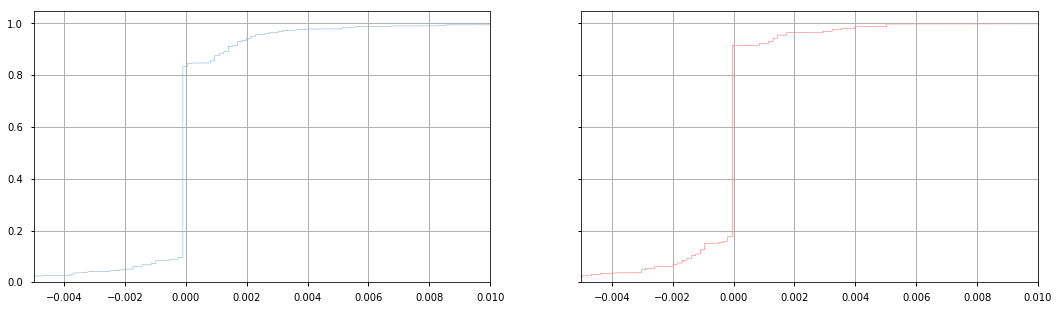
\includegraphics[width=1\linewidth]{images/KS_CER_DN_18_CUMUL.png}    
    \end{center}
    \caption{Comparison of distributions between the weekend and weekday population for \texttt{CER\_DN\_18H} using cumulative distributions (the left curve representing the weekend population)}
    \label{KS_CER_DN_18_CUMUL}
\end{figure}

Figures~\ref{KS_CER_UP_12} and \ref{KS_CER_UP_6} show the distribution of the top 2 p-values. It isn't so obvious from a graphical perspective that these two variables are sampled from different distributions even if we can see that during the week the two features are more likely to be zero (as indicated by the high bar centered in 0 on the right plots). 

For the third feature, the initial plot (cf. Figure~\ref{KS_CER_DN_18}) was not very informative, therefore we decided to switch to a cumulative distribution plot. Again figure~\ref{KS_CER_DN_18_CUMUL} doesn't show much evidence of the two underlying distributions being different.

This concluded our introductory analysis using the KS test. Apparently we cannot show evidence of the two distributions being drastically different. This motivated us to switch to a different test. 

\subsubsection{High Dimensionality Hypothesis Testing}
The previous test, put aside the fact that it wasn't very conclusive, only takes into consideration each individual feature. We are indeed interested in knowing whether the vectors differ between weekend and weekdays. 

High dimensional computation is one of the challenges that is still at the center of research and we studied many papers~\cite{min_energy,two_sample_equality,dimensional_object,energy_test} to determine a proper test to use in our use case. The energy test based on bootstrapped test-statistic estimation seemed promising as it would help us efficiently run such tests.

\paragraph{Theoretical Concept}  
Suppose that we have $X_{1},...,X_{n_1}$ and $Y_{1},...,Y_{n_2}$ independent random samples of random vectors in $\mathbb{R}^d$. Let $\mathcal{A}$ and $\mathcal{B}$ be two populations of samples of respective size $n_1$ and $n_2$ such that $n=n_1+n_2$. The article proposes a new test statistic, the energy:

\begin{align}
	\mathcal{E}_{n_1,n_2} = e(\mathcal{A},\mathcal{B}) = \frac{n_1 \times n_2}{n} ( & \frac{2}{n_1\times n_2} \sum_{i=1}^{n_1}\sum_{m=1}^{n_2}||X_i-Y_m||\\ 
	&- \frac{1}{n^2}\sum_{i=1}^{n_1}\sum_{j=1}^{n_1}||X_i-X_j||\\ 
	&- \frac{1}{n^2}\sum_{i=1}^{n_2}\sum_{j=1}^{n_2}||Y_i-Y_j||)\\
\end{align}

Suppose that $X,X',Y,Y'$ are independent random vectors of $\mathbb{R}^d$ with finite expectations such that $X \buildrel d \over = X'$ and $Y \buildrel d \over = Y'$, then:

\begin{equation}
	2 E||X-Y||- E||X-X'||- E||Y-Y'|| \ge 0
\end{equation}

and the equality holds if and only if X and Y are equally distributed. Therefore we expect the energy statistic to be large if the null hypothesis can be rejected.

\paragraph{Practical Implementation}
Let $\alpha$ be the significance level. We will sample B bootstrap samples $W_1^{(b)},...W_n^{(b)} \quad \forall b \in \{0,...,B\}$ such that $(B+1)\alpha$ is an integer. $W$ is the random variable obtained by sampling from a $X$ and $Y$ with respective probabilities\footnote{This means that we pool all the elements of $X$ and $Y$ in a single set and sample uniformly at random from this set.} $n_1/n$ and $n_2/n$. 

For each bootstrap sample $b$, we compute $\mathcal{E}_{n}^{(b)}$ determined by k samples:

\begin{equation}
\begin{cases}
	\mathcal{A}_1^{(b)} = \{W_1^{(b)},....W_{n_2}^{(b)}\}\\
	\mathcal{A}_2^{(b)} = \{W_{n_1 + 1}^{(b)},....W_{n}^{(b)}\}
\end{cases}
\end{equation}

Then the bootstrap estimate of $P_n(\mathcal{E}_{n} \le t)$ is $\frac{1}{B} \sum_{i=1}^B I(\mathcal{E}_{n}^{(b)} \le t)$.

Put in simple words, we will compute the energy statistic for the original population segmentation giving us $t_\text{obs}$. Then $B$ times, we will create two new populations by sampling from the pooled population. On each bootstrap we will compute the energy bootstrap estimate. We will then check the ratio of bootstrap estimates that are lower than $t_\text{obs}$, this will give us the p-value. 

Because we will compute the distance between two vectors of the pooled population many times, we will start by computing the distance matrix that provides the distance between any two pair of vector from the pooled population.

\paragraph{Results}
The dataset used for this test was composed of 44,556 samples from the weekday population against 17,740 for weekends, therefore the distance matrix would be composed of 790,423,440 entries, which isn't easy to work with on a personal computer due to memory requirements. We derived three strategies in order to perform the test:
\begin{itemize}
	\item \textbf{Averaging vectors over day type}: we average for each MAC the vector over all vectors from the weekend and then all vectors from the week. This provides two populations of equal sizes where there is a single entry per MAC in each.
	\item \textbf{Sampling populations}: we sample from each population without replacement in order to obtain smaller populations. 
	\item \textbf{Multiple samples}: in order to obtain a better estimate we run the previous strategy on ten different samples. This will give us 10 different p-values that we can average to obtain a stronger estimate.
\end{itemize}

\begin{table}[h]
\begin{center}
\begin{tabular}{c r r r l}
\hline
\textbf{Strategy} & \textbf{Observed} & \textbf{Limit} & \textbf{p-value} & \textbf{Decision}\\ 
\hline\hline
Day type average &  $87340.19$ & $71.00$ & $0$ & Reject $H_0$\\
\hline
Subsampling &  $57526.91$ & $86.97$ & $0$ &  Reject $H_0$\\
\hline
Repeated subsampling &  (avg)$58771.53$  & (avg)$100.12$ & $0$ &  Reject $H_0$\\
\end{tabular}
\end{center}
\caption{\label{hyp_test_res}Energy test results for different strategies}
\end{table}

Table~\ref{hyp_test_res} presents the result obtained with this test. The results show that we can reject the null hypothesis at confidence level $>99.99\%$. Therefore we are confident that weekend and weekday's vectors have distinct underlying distributions. To increase our confidence in the test we performed the same test but this time by using two populations generated from exclusively weekday/weekend populations. We expect these tests not to reject the null hypothesis at reasonable confidence levels.

\begin{table}[h]
\begin{center}
\begin{tabular}{c r r r l}
\hline
\textbf{Strategy} & \textbf{Observed} & \textbf{Limit} & \textbf{p-value} & \textbf{Decision}\\ 
\hline\hline
Subsampling (week only) &  $21.15$ & $182.55$ & $0.9394$ & Cannot reject $H_0$\\
\hline
Subsampling (weekend only) &  $18.99$ & $79.40$ & $0.7374$ & Cannot reject $H_0$\\
\hline\hline
Repeated subsampling (week only) & (avg)$32.49$ & $130.61$ & $0.6929$ & Cannot reject $H_0$\\
\hline
Repeated subsampling (weekend only) & (avg)$34.83$ & $76.463$ & $0.4363$ & Cannot reject $H_0$\\
\end{tabular}
\end{center}
\caption{\label{hyp_test_control}Energy test results for control experiments}
\end{table}

Table ~\ref{hyp_test_control} shows that the test doesn't reject the null hypothesis when we are sampling for each distinct population which increases our confidence in results. 

\vspace{1\baselineskip}A preliminary step was followed to mitigate this phenomenon. We constructed for each vector a categorical variable \texttt{WEEKDAY}. It gives us the information regarding what day of the week is Day\textsubscript{0}. It is important to note that "data cannot prove correctness of a theory (hypothesis), because we can always imagine that future data or a new experiment might undermine it, but data can falsify a theory"\footnote{As presented in the "Probabilities and statistics" class given by Pr. Davison (slide 348 of the course book).}. We cannot prove that the two distributions here are different, we can only reject that they are identical at a particular confidence level. 

\subsection{Exploratory Data Analysis}
EDA allows us to gain insights on the data that we are working with. Our problem makes such analysis complex as we are working with 290 features. We decided to only look at particular characteristics of the dataset. We started with a standard data report to understand the distribution of features. We followed with an analysis of the NULL values. Finally, we investigated the correlation among components to ensure that we discard components that do not add value. 

\subsubsection{Data Report}
With 291 components in our vectors, it would have been quite repetitive to produce meaningful plots for each of them. Hopefully the data science team has developed a tool that produces such exploration automatically. In the appendix~\ref{sec:continuous} and~\ref{sec:categorical} we have provided some plots constructed by this package. 

The number of such plot prevents a comment for each of them but we would like to make a few remarks:
\begin{itemize}[noitemsep,topsep=0pt]
	\item Many features are highly skewed in their center, which could be explained by the fact that we expect signal values not to fluctuate too much and therefore the relative difference between two consequent aggregates is expected to be close to zero.
	\item Most features that are not from the \texttt{MISS\_*} type are approximately normally distributed. 
	\item The \texttt{SEQ\_ID} is approximately uniform which supports our confidence in this sequence number to be rarely forming gaps as we argued in section~\ref{subsec:data_sampling}.
\end{itemize}

The report also performed some other analysis but it wasn't particularly relevant due to the size of vectors. As an example a graphical correlation analysis would be unusable here. Hence we performed it in another way. 

\subsubsection{Null Value Analysis}
As we previously mentioned it in section~\ref{subsubsec:constructed_features}, missing values carry a lot of sense for us. Because we have aggregated the data at the database level, we are forced to perform this analysis on the aggregated measurements. This means that we are not necessarily showing the true underlying patterns. 

Indeed, an aggregate is null if and only if all the aggregated measurements are also null\footnote{By design of Oracle's average function that ignores missing values.}. Also the relative difference between two values is null if one of the two components at least is null itself. 

In order to give a high-level view of null values we used a package that allows us to produce a graphical representation of null values. Figure~\ref{white_matrix} illustrates the existence of patterns in missing values. Given the number of columns it is complex to analyse such pattern with that particular graph. 


\begin{figure}[ht]
    \begin{center}
    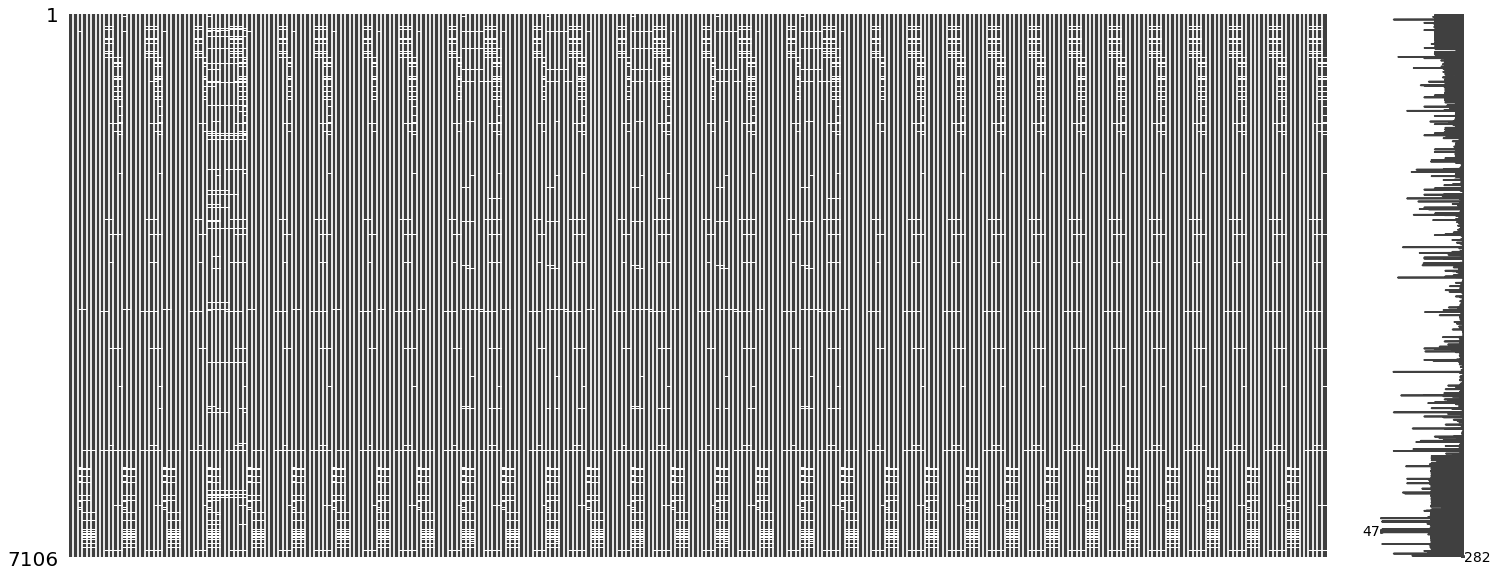
\includegraphics[width=1\linewidth]{null_white_pattern}
    \end{center}
    \caption{Matrix representing missing values as white cells on the dataframe}
    \label{white_matrix}
\end{figure}

We therefore used a dendogram. It displays variable completion, revealing trends deeper than the pairwise ones visible in a correlation heat map. Cluster leaves which are linked together at a distance of zero fully predict one another's presence: one variable might always be empty when another is filled, or they might both be always filled or both empty, and so on.

\begin{figure}[ht]
    \begin{center}
    
\includegraphics[width=1\linewidth]{dendogram_part}
    \end{center}
    \caption{Data completion dendogram (partial)}
    \label{dendogram}
\end{figure}

As the graph is too long to fit on a page, only a fraction of it is presented in the figure~\ref{dendogram}. What is interesting is to see that measurements are grouped by days at which they are aggregated but also sometimes by the fact that they are taken at the CMTS or CPE level. 

Regarding the level of collection of the data, this data completion correlation could indicate some data polling issues on particular period of time. Also the fact that multiple measurements have data completion correlation when computed on the same time window could confirm the intuition that measurements are most probably missing when the CPE is offline. 

This analysis only gives coarse grain patterns as it would be complicated to look at every single clustering to determine some underlying pattern. Therefore we moved to a correlation analysis on the feature space not only taking into account data completion. 

\subsubsection{Feature Elimination}
By analysing highly correlated variables our aim was to reveal features that do not add much usable information for further works and could be discarded. Then we also decided to determine whether some component of the vector was particularly inexpressive. 
 
\paragraph{Correlated Features}
As we started the correlation analysis, we discovered that some features were exactly identical for every single sample. This proved to be a mistake during the data collection process. For the \texttt{MISS\_*} features, we have added two features, namely \texttt{MISS\_\{mes\}} and \texttt{MISS\_\{mes\}\_1d} that both represented the ratio of missing values over the past day. Hopefully this could easily be fixed by deleting the duplicate when importing the data (correcting the data collection package would have invalidated all data collected so far so we decided to prefer a fix at import time).

Once this was fixed, we could look at highly correlated features. This revealed 48 groups of features that had a correlation higher than $0.9$. We split these groups in two. First, those that correspond to two or more measurements that are correlated for every single time aggregate. This is most likely showing that original measurements are correlated. That yielded 4 groups of correlated measurements:
\begin{itemize}[noitemsep,topsep=0pt]
	\item \texttt{CMTS\_MS\_UTILIZATION\_UP} $\equiv$ \texttt{CMTS\_UTILIZATION\_UP}
	\item \texttt{MISS\_PCT\_TRAFFIC\_SDMH\_UP}  $\equiv$ \texttt{MISS\_PCT\_TRAFFIC\_DMH\_UP}
	\item \texttt{MISS\_SNR\_DN}  $\equiv$ \texttt{MISS\_RX\_DN}  $\equiv$ \texttt{MISS\_TX\_UP}
	\item \texttt{MISS\_SNR\_UP}  $\equiv$ \texttt{MISS\_RX\_UP}
\end{itemize}
In order to decide whether we could discard all but one feature of each of these groups, we plotted for each time aggregate each measurement of the correlation group against each other. For each group these plots displayed strong evidence that the measurements are nearly identical but also Pearson and Spearman correlations were always above $0.98$. Therefore we always discarded all measurements but one from the correlation group in order to discard measurements that would not add information. Table~\ref{correlation_insp} only presents such plot for the first group of variables, for other groups the results can be found in the final notebook and are similar to the one we chose to display.

\begin{figure}[h]
\begin{center}$
\begin{array}{ccc}
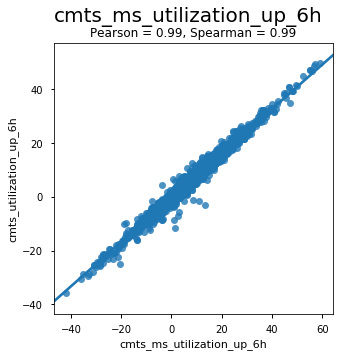
\includegraphics[width=1.5in]{correlation-1} &
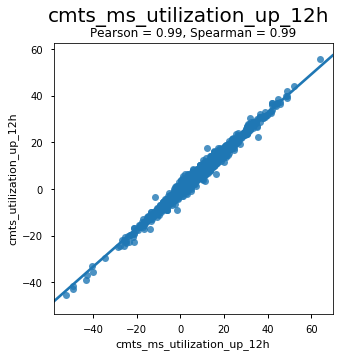
\includegraphics[width=1.5in]{correlation-2} &
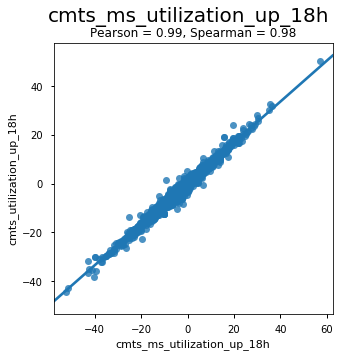
\includegraphics[width=1.5in]{correlation-3}\\
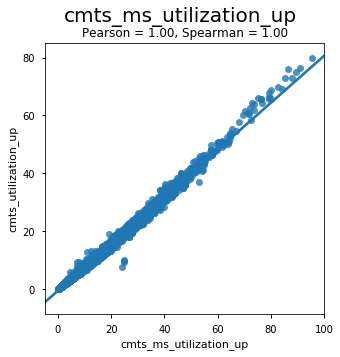
\includegraphics[width=1.5in]{correlation-4} &
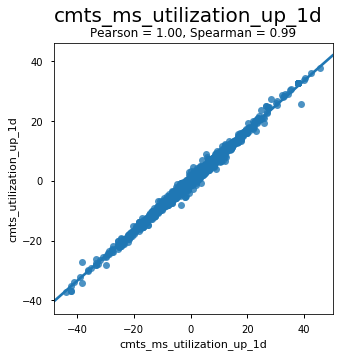
\includegraphics[width=1.5in]{correlation-5} &
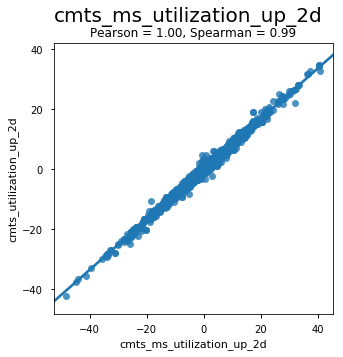
\includegraphics[width=1.5in]{correlation-6}\\
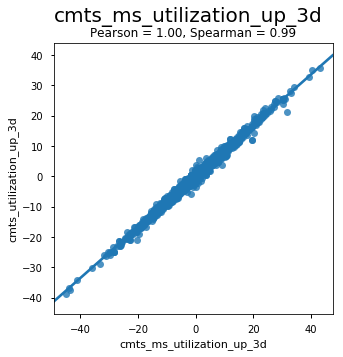
\includegraphics[width=1.5in]{correlation-7} &
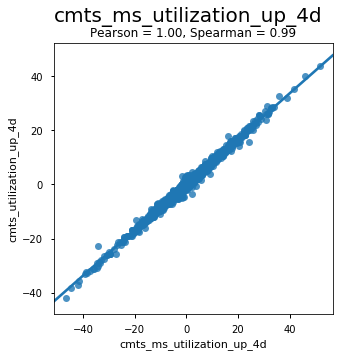
\includegraphics[width=1.5in]{correlation-8} &
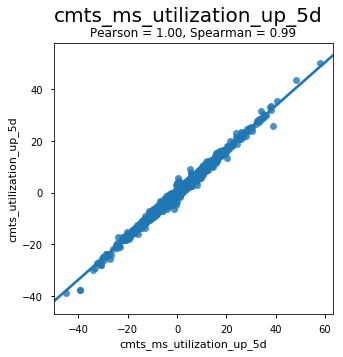
\includegraphics[width=1.5in]{correlation-9}\\
\end{array}$
\end{center}
\caption{\label{correlation_insp}Graphical correlation inspection for \texttt{CMTS\_MS\_UTILIZATION\_UP} $\equiv$ \texttt{CMTS\_UTILIZATION\_UP}}
\end{figure}

Then we investigated 3 groups of features that were not correlated for every time aggregate:
\begin{itemize}[noitemsep,topsep=0pt]
	\item \texttt{MISS\_RX\_UP\_24H} $\equiv$ \texttt{OFFLINE\_PCT\_24H}
	\item \texttt{MISS\_RX\_UP\_6H}  $\equiv$ \texttt{OFFLINE\_PCT\_6H}
	\item \texttt{MISS\_SNR\_DN}  $\equiv$ \texttt{MISS\_RX\_UP}
\end{itemize}
Figure~\ref{almost_correlation_insp} shows scatter plots (using hex bins to show density at particular points) of each feature plotted against the one that it seems correlated to. We see that some correlation pattern exists. Nevertheless we decided not to discard any of these features. Indeed, graphical correlation isn't as explicit but also because the correlation on particular time aggregates doesn't explain a correlation at the raw measurement level. These particular cases could be handled either by the model that will not use the features or by a dimensionality reduction techniques at a later stage.

\begin{figure}[h]
\begin{center}$
\begin{array}{ccc}
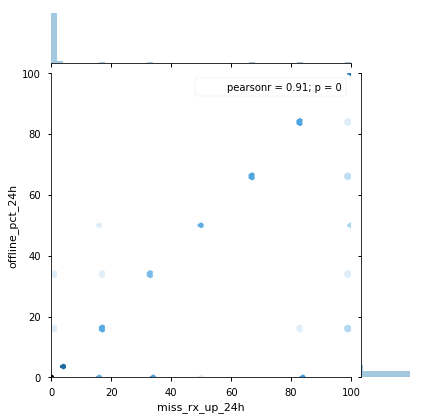
\includegraphics[width=2in]{almost_corr_1} &
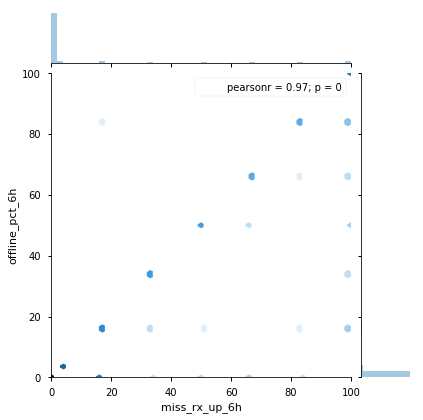
\includegraphics[width=2in]{almost_corr_2} &
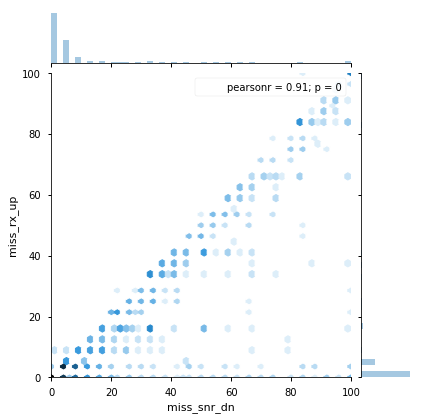
\includegraphics[width=2in]{almost_corr_3}
\end{array}$
\end{center}
\caption{\label{almost_correlation_insp} Graphical correlation inspection for features that are not correlated for every time aggregate}
\end{figure}

\paragraph{Near Zero Variance}
By inspiration from the R package called caret\footnote{\url{https://www.rdocumentation.org/packages/caret/versions/6.0-80/topics/nearZeroVar}}, we also investigated features that do not have much variance. To detect such features we focused on those that satisfy any of the following two characteristics:
\begin{itemize}[noitemsep,topsep=0pt]
	\item The most common value is represented by more than 99\% samples (near zero variance predictors)
	\item Very few unique values w.r.t the number of samples (by default $<10\%$) and the frequency of the most common value to the frequency of the second most common value is large (by default $>95/5$)
\end{itemize}

Figure~\ref{nearzerovar} presents the features that we investigated. As we should explain in Section~\ref{sec:datapreprocessing}, \texttt{model\_i} are features that encode the \texttt{HARDWARE\_MODEL} and therefore for such variables we expect low variance. Other variables are discrete and therefore as a second intuition we wondered if by discarding these features we would not be shaving off exactly the features that give us outliers. Some graphical investigation seems to indicate that most of these features were flagged du to the high skew in their center as we already witnessed it in the data report. This investigation yielded no interesting results. 

\begin{figure}[ht]
    \begin{center}
    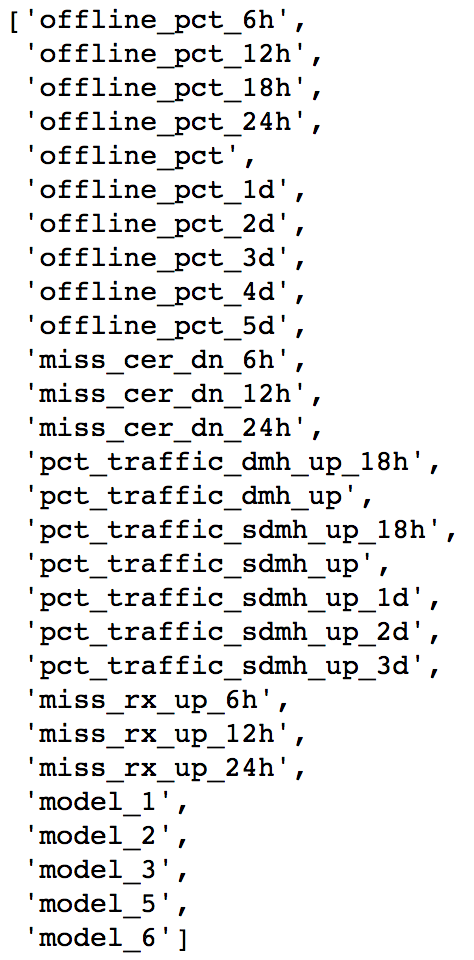
\includegraphics[scale=0.5]{nearzerovar}
    \end{center}
    \caption{Features flagged by the \texttt{NearZeroVar} function (suspected of having low variance)}
    \label{nearzerovar}
\end{figure}

\vspace{1\baselineskip}
The intermediary analysis allowed a better grasp of the characteristics of the dataset. Thanks to a high-dimensional test we determined that weekends had an influence on vectors and tried to mitigate this influence by adding a new feature. Then we explored our dataset to find out about the distribution of features as well as their correlation. 

\section{Data Preprocessing}
\label{sec:datapreprocessing}
Data preprocessing steps are necessary for most of models to perform well. We will discuss the different strategies that have been used in order to preprocess the dataset for classification. In the following paragraphs we will consider $x_i^{(1)},...,x_i^{(d)} \quad \forall i\in \{1,...N\}$ (number of samples) and  $\forall d \in \{1,...D\}$ (dimension of each sample) to be our input and $y_i \quad \forall i\in \{1,...N\}$ to be our target. Finally we will denote by $\hat{y}_i \quad \forall i\in \{1,...N\}$ the predictions of our model.

\subsection{Target Binarization}
At the start of the project we considered the possibility of performing a multi-class classification. This explains our attention to the correctness of labels. That would allow to achieve other business goals as providing a new tool to diagnose CPE problems and automatically determine the good flow to service the customer. Nevertheless, an initial approach would be to start with a binary classification. Therefore rather than focusing on labels we would focus entirely on whether the CPE is failing or not (which we indicate by transforming the \texttt{MILESTONE\_NAME} feature into 1 and 0 to indicate if it is respectively sick or not.
 
\subsection{One-Hot Encoding}
\label{subsec:one_hot}
As described by the collaborative encyclopedia~\cite{wiki:onehot}, one hot encoding allows to describe a categorical feature by creating as many features as there are categories and setting exactly one feature to the high state (1) when the original feature lies in this particular category. This is a desirable modification as some models heavily relies on the value of a particular feature. In our case we have two categorical features \texttt{WEEKDAY} and \texttt{HARDWARE\_MODEL}. 

If we consider a simple linear regression, it will compute a weight $\omega_i^{(k)}$ to each feature $x_i^{(1)},...,x_i^{(d)}$ such that $\hat{y}_i=\sum_{k=1}^d{\omega_i^{(k)}\times x_i^{(1)}}$ (the linear combination determines the predicted label). Hence one can see that for a categorical feature as \texttt{WEEKDAY} it wouldn't make sense to care about its absolute value but rather what is the value it takes. Hence we created two new groups of features \texttt{wk\_\{i\}} and \texttt{model\_\{i\}}.

\subsection{Missing Value Imputation}
Because a machine learning algorithm works with an underlying mathematical model it requires numbers to perform correctly. This is why we need to transform missing values. There exist many imputation techniques, nevertheless in our case we do not need too much reflexion regarding the one to use. Indeed, as we discussed in section~\ref{subsubsec:constructed_features}, we have added a feature that provides the information of missing values such that we do not lose it. 

Our aim is to "hide" missing values as well as we can. Because of our scaling choice that we should discuss in next subsection we will replace each missing value by the feature's mean.


\subsection{Scaling}
This addresses the same problem as discussed in section~\ref{subsec:one_hot}. We wish features to have comparable scales in order to not bias our models toward a particular feature importance consideration. This is not necessary for each model but it is desirable to apply it for model exploration to be able to black box test each model. We will discuss later on its usefulness for our picked models. 

\begin{table}[h]
\begin{center}
\begin{tabular}{c c p{80mm}}
\hline
\textbf{Strategy} & \textbf{Scaled Features} & \textbf{Comment} \\ 
\hline\hline
Log Scaling & $x_i'=\log(x_i)$ & Good for heavy tailed features (Distribution with higher probability of getting large values)\\
Min-Max Scaling & $x_i' = \frac{x_i - min}{max-min}$  & May scale typical values to small intervals in case of outliers\\
Standardisation & $x_i' = \frac{x_i - \mu_i}{\sigma_i}$ & Very meaningful in case of normally distributed features and more resistant to outliers. (Where $(\mu_i, \sigma_i)$ are the mean and standard deviation of the feature)
\end{tabular}
\end{center}
\caption{\label{scaling}Scaling strategies}
\end{table}

Out of the three main strategies that we considered and presented in table~\ref{scaling}, we decided to standardise features. This is coherent with the data report that displays many normally distributed features but also because many features contain outliers.

\subsection{Dimensionality Reduction}
The curse of dimensionality~\cite{wiki:curse} is an important problem in cases that are similar to ours. Indeed, we are here working with many features and as many models rely on the notion of distance they might be ineffective due to meaninglessness of such notion in high-dimensional spaces (which is also why we had to use specific techniques in section~\ref{subsec:influence}).

To fight high dimensionality of the feature space different techniques exist and we experiment with two of them.

\subsubsection{Principal Component Analysis}
PCA is a popular dimensionality reduction technique~\cite{pca} that compresses the data to display it in a more meaningful representation which relies on the use of singular vector decomposition. It can be sometimes misleading as we often talk about PCA's number of components used. These components should not be confused with features, these are rather the number of vectors that will compose the new base to represent our data. 

\begin{figure}[ht]
    \begin{center}
    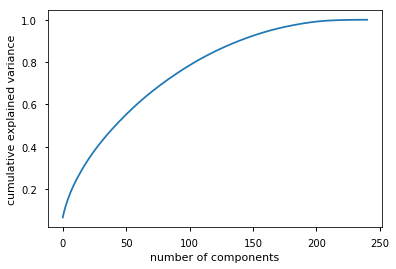
\includegraphics[scale=0.5]{pca_var}
    \end{center}
    \caption{Tradeoff between the level of variance explained and the number of components of PCA}
    \label{pca_var}
\end{figure}

Figure~\ref{pca_var} illustrates how by considering an increasing number of components we increase the cumulative explained variance. To leverage the power of PCA's compression we decided to retain 95\% of the variance with PCA. Again this could be more finely tuned but was chosen as a baseline. 

\subsubsection{Linear Discriminant Analysis}
LDA~\cite{wiki:lda} uses an extra piece of information. It uses the labels of samples in order to find a single number combination of features that separates the most classes. The resulting combination can be used already as a linear classifier but is most commonly used solely as a dimensionality reduction technique. Because it gives weight to each feature, it may not be necessary to scale them beforehand. 

\vspace{1\baselineskip}
The first two preprocessing steps, Binarization and one hot encoding are grouped together as they are performed on all samples of the dataset. On the other hand, dimensionality reduction, imputing and scaling have to compute statistics on the training set that are applied both on the training and testing set. Therefore they need to be done when the model is fitted/train and will be grouped with the classifier. For the purpose of efficient implementation, we used a component proposed by scikit-learn called pipeline\footnote{\url{http://scikit-learn.org/stable/modules/generated/sklearn.pipeline.Pipeline.html}}. It allows to group different steps into a single object that can then be used as black box for the ML part. 

\section{Clustering Attempt}
Considering some of the characteristics of the way that we label our samples we thought that clustering coupled with some expert help at analysing these clusters would help us enhance labeling. Indeed, customer calls cannot be considered as the strongest indicator of whether a particular CPE is failing. This is due to multiple reasons. First of all, we cannot be sure that every customer has the same way of dealing with CPE failures. Some might call the service center in the following minutes because they are using the service at the moment of failure, some may fix the problem themselves by rebooting the CPE or some other quick fix. Hence we cannot be sure that a particular problem will be flagged in the same timeframe than another instance of that problem, or that it will be flagged at all. Secondly, we used a database that was not designed to answer this project's requirements and therefore we had to filter down the data and may be discarding many 'sick' CPEs for the sake of problem labeling precision. 

Therefore by clustering our vectors we aimed at unveiling the underlying structure that would indicate failures. In the case where we would have found a clustering displaying satisfying structure we could have gone to Jonas Staempfli in order to look with him at the CPEs that are grouped together to determine.

In this section we will present the different methods that have been tested to cluster the data, then we will discuss the result of such clustering and try to explain why we think it isn't usable.


\subsection{Exploring}
We started with the most popular and simple model: K-Means clustering. Many clustering algorithm exist but often require to tune multiple parameters in order to obtain decent results which motivated our choice of the simplest clustering algorithm.

\subsubsection{Evaluating Performance}
Because clustering is unsupervised it is usually difficult to evaluate its performance. In our case, we do have the labeling but are interested in improving such labeling forcing us not to rely entirely on it. Extending our existing labeling by propagating labels inside clusters based on majority votes could lead to a serious overestimation of the performance of a future classifier (it would be as if we decided to change the labels of samples that are classified as false negatives or false positives such that they are now classified correctly).

\paragraph{Silhouette Analysis}
A silhouette analysis is used to assess the structure of a clustering. It uses a measure that translates how close each point in one cluster is to points in the neighbouring clusters. This measure ranges in $[-1,1]$ and is called a \textbf{silhouette coefficient}. 

Silhouette coefficients close to 1 indicate that the sample is far away from the neighbouring clusters. A value of 0 indicates that it lies on the decision boundary between two clusters and a value near -1 indicates that the sample might have been assigned to the wrong cluster.

Using these coefficients, we can decide on the most appropriate hyper-parameter like $k$ (number of clusters) in our case. We create plots were we show ordered coefficient values for all points in each cluster. The interpretation of such plot resides in the fact that:
\begin{itemize}
	\item we wish to avoid having certain cluster that have below average silhouette scores (as indicated by the red line)
	\item we wish to have homogeneous size in the silhouette plots (when the classes are supposed to be balanced, which is a basic assumption of K-Means)
\end{itemize}

But also we can use the average of silhouette coefficients in order to determine the quality of the model~\cite{silhouette}:
\begin{itemize}[topsep=0pt,noitemsep]
	\item $[1.0,0.7)$ : A strong structure has been found
	\item $[0.7,0,5)$ : A reasonable structure has been found
	\item $[0.5,0.25)$ : The structure is weak and could be artificial. Try additional methods of data analysis
	\item $< 0.25$ : No substantial structure has been found
\end{itemize}

\paragraph{Elbow Method}
Another method that we tried to use was the elbow method. It uses a plot of the Sum of Squared Error (SSE) against the number of clusters to determine the optimal $k$. The point where the plot starts flattening significantly (forming an elbow) indicates the optimal number of clusters. 

\subsubsection{Initial Results}
Using only preprocessing (scaling and imputation), we used a sample of the data that was collected up to the 27\textsuperscript{th} in order to attempt to cluster. 

\begin{table}[h]
\begin{center}
\begin{tabular}{c c c}
\hline
\textbf{$k$} & \textbf{(Scaling+Imputing)} & \textbf{(+PCA)}\\ 
\hline\hline
2 & \textbf{0.2837} & \textbf{0.4354}\\
3 & 0.0235 & 0.0928\\
4 & 0.1524 & 0.2033\\
5 & 0.0112 & 0.0636\\
6 & 0.0120 & 0.0160\\
7 & 0.0219 & 0.0491\\
\end{tabular}
\end{center}
\caption{\label{silh_scor_simple}Average silhouette scores for different number of clusters with scaled and imputed data}
\end{table}

\begin{figure}[ht]
    \begin{center}
    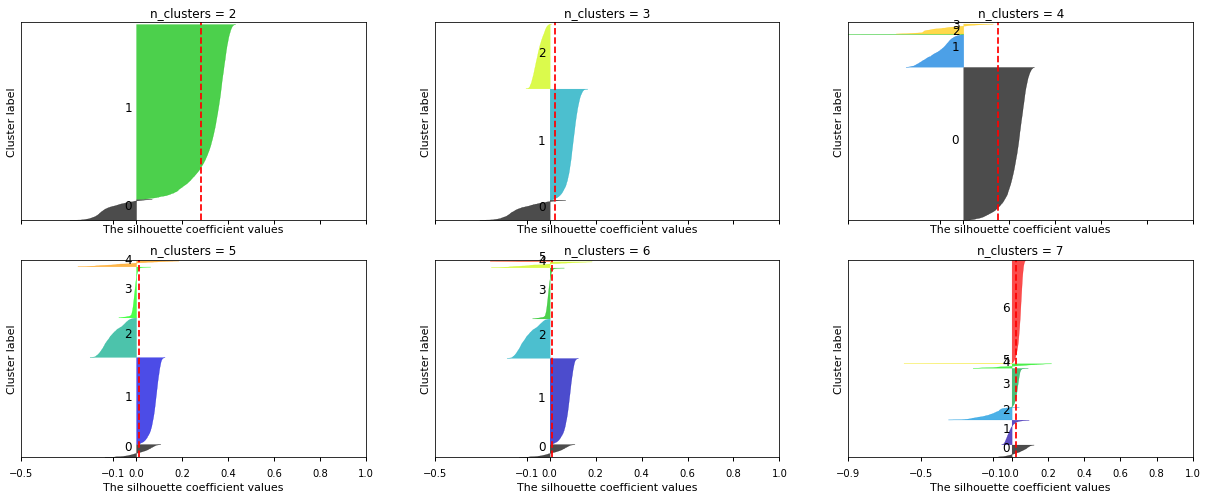
\includegraphics[width=1\linewidth]{clust_simple}
    \end{center}
    \caption{Silhouette analysis with preprocessing step}
    \label{clust_simple}
\end{figure}

Figure~\ref{clust_simple} and table~\ref{silh_scor_simple} display the result of such exploration. We see that the score never reaches levels that could enhance our confidence and the clustering with the highest silhouette score being $0.2837$. We tried to apply a PCA retaining 95\% of the variance in the hope to improve the scores by fighting the curse of dimensionality. But as it can be seen in table~\ref{clust_pca}, even the highest silhouette score still lies under satisfying levels and the silhouette plots confirm that this clustering isn't well structured.   

\begin{figure}[ht]
    \begin{center}
    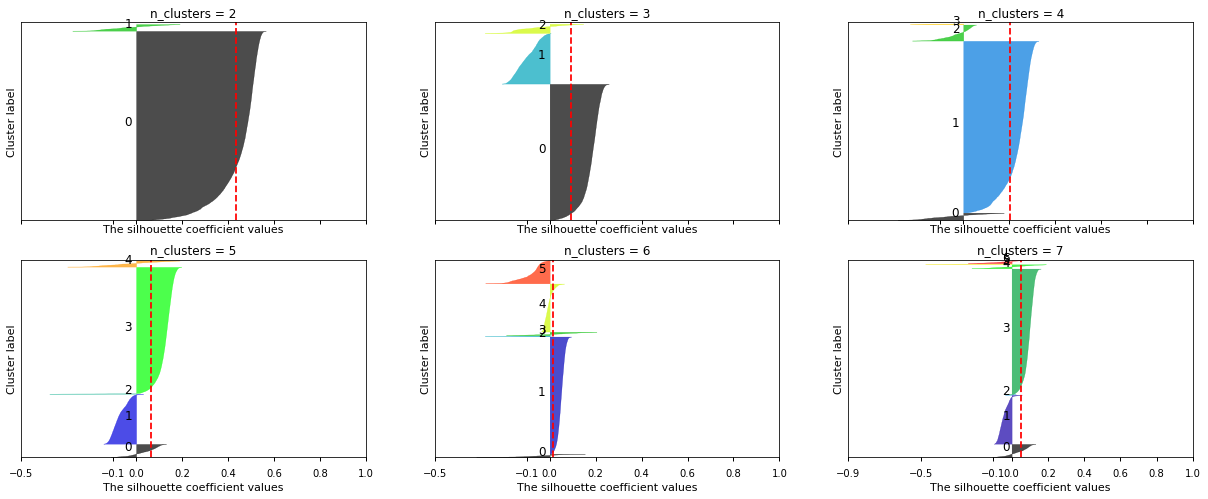
\includegraphics[width=1\linewidth]{clust_pca}
    \end{center}
    \caption{Silhouette analysis with a PCA (on top of preprocessing) retaining 95\% (yielding 165 components)}
    \label{clust_pca}
\end{figure}

We also tried wider ranges of clustering without much success, the scores still indicating that our clustering wasn't successful. Also what surprised us was that running multiple times the same algorithm on the same data would yield very variable results and therefore decreased our confidence in such model. 

We therefore tried to use additional tricks to improve our score and hopefully at the same time obtain more stable models. 

\subsection{Improving Scores}
As an extra performance metric, we decided to look at binary clustering as a prediction. That is, we would predict a cluster based on the majority class of labels in it. That would help us get metrics that we are more familiar with such as precision or recall but again this must be considered with extreme care as it doesn't translate the structure of the clustering (whether it is due to pure luck or not) and it relies on the existing labeling.

\subsubsection{Balancing the Dataset}
K-means is based on the assumption that clusters are of similar sizes, therefore we tried to balance the classes. This technique could seem incompatible with our aim to correct the labels. Indeed, by balancing we may discard false negatives from the 'healthy' class. But if we manage to find a correct clustering we could later use the cluster centers in order to cluster all the points using their distance to each center. 

Different techniques of data balancing exist but given our choice at the database level to subsample the sick class we remained in the same strategy at the data analysis level. 


\begin{figure}[ht]
    \begin{center}
    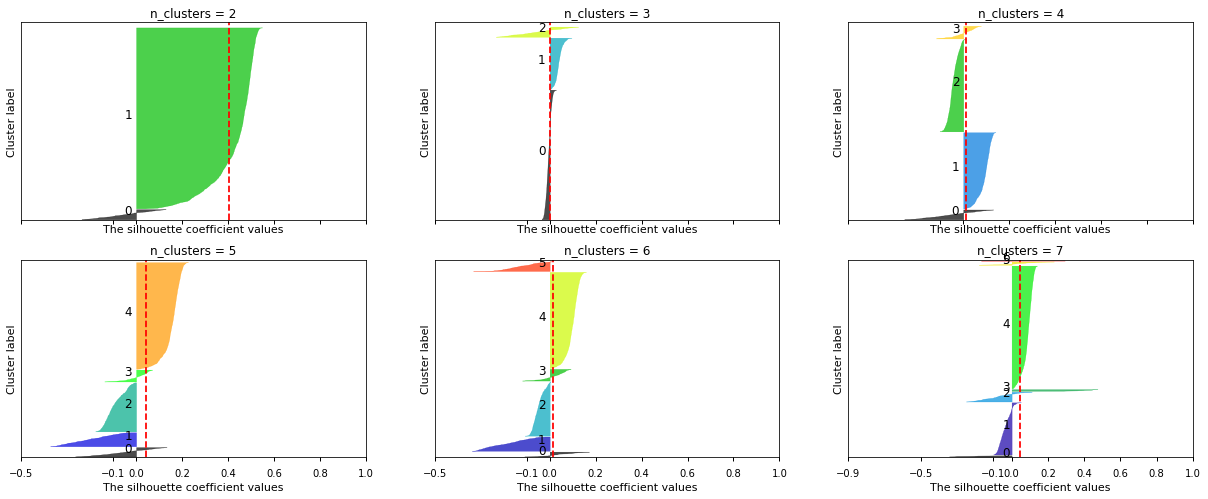
\includegraphics[width=1\linewidth]{clust_balanced}
    \end{center}
    \caption{Silhouette analysis with balanced class (on scaled and balanced data)}
    \label{clust_bal}
\end{figure}

One can observe on figure~\ref{clust_bal} that the scores are still fairly low. If we look closer at the binary clustering that is the most promising score of 0.4065, we obtain table~\ref{clust_clas}. It shows that either we are very wrong in the way we label data or there isn't a structure that can be exploited by K-Means.

\begin{table}[h]
\begin{center}
\begin{tabular}{c c c c c}
\hline
\textbf{Cluster interpretation} & \textbf{Desc} & \textbf{Counts} & \textbf{Label Proportion} & \textbf{Cluster proportion}\\ 
\hline\hline
\multirow{2}{*}{Healthy}  	& True negatives & 1140 & 97.94\% & 51.65\%\\
						  	& False negatives & 1067 & 91.68\% & 48.35\%\\
\hline
\multirow{2}{*}{Sick}  	& False positives & 24 & 2.06\% & 19.83\%\\
						  	& True positives & 97 & \textbf{8.33\%} & \textbf{80.17\%}\\
\end{tabular}
\end{center}
\caption{\label{clust_clas}Binary clustering interpreted as binary classification (balanced classes). On the sick class, we observe Recall$=8.33\%$ and Precision$=80.17\%$}
\end{table}

\subsubsection{Combining Dimensionality Reduction With Balanced Classes}
Because the score increased both thanks to class balancing and dimensionality reduction we combined both. We evaluated the average silhouette score for different levels of retained variance as shown in figure~\ref{clust_pca_diff_lev}. Even though we increased the average silhouette score of binary clustering we are still not obtaining scores that would allow us to present the clustering to the expert and check its output. 

\begin{figure}[ht]
    \begin{center}
    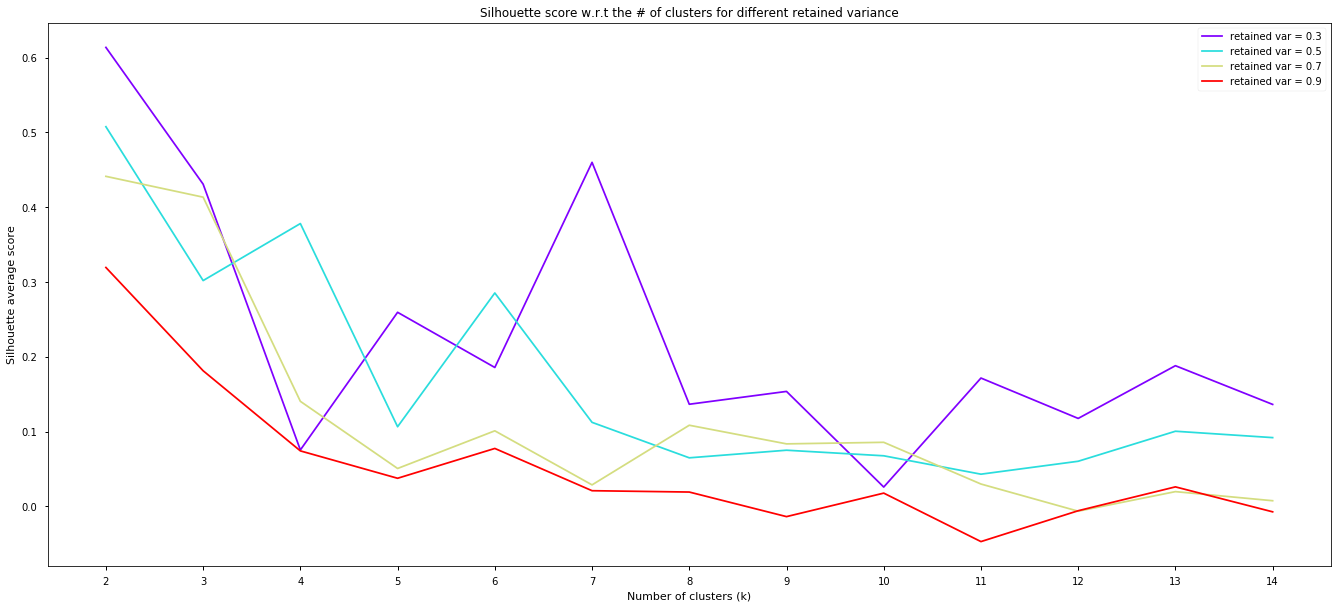
\includegraphics[width=1\linewidth]{clust_pca_diff_lev}
    \end{center}
    \caption{Average silhouette score for different levels of retained variance and different numbers of clusters (PCA+balanced classes)}
    \label{clust_pca_diff_lev}
\end{figure}

An attempt was also made at using LDA in combination of balanced classes with promising results on binary classification with $(R=50.515\%,P=81.667\%)$, unfortunately the average silhouette score of 0.1201 again revealed the poor structure that this clustering displayed and was hence abandoned. 

\vspace{1\baselineskip}
After this initial attempt at clustering, in concert with the business intelligence team we decided to move to classification. First of all, we couldn't display any clustering model that would be trustworthy. Also the lack of resources in the HFC support team made it complicated to check model outputs. 

To explain the difficulty experienced in our exploration of a correct clustering technique we thought of many reasons. The curse of dimensionality clearly plays a role in this as the notion of distance that is used both in the clustering algorithm and the scoring may be unusable. But also as a given problem may have different fixes, it would also be possible that 'symptoms' diverge with great magnitude preventing any clustering to reveal the underlying pattern. 

We focused back on classification as it usually relies on more complex models that can capture these differences in symptoms but also because the goal of the project is to provide a Proof-of-Concept to push the launch of a business project. Once such project goes live, the data can be sensibly enriched and cleaned to avoid the need for clustering as we will emphasise in section~\ref{sec:improving}. 

\section{Failure Prediction}
The predictions were the final goal of the project and our aim was to show that indeed we could predict the failures of some CPEs. As illustrated in previous steps, because the data could have been much improved and as models are only as good as the data they are fed, we focused on our top 'sick' predictions rather than focusing on the whole classification. This choice was again made after discussions with the supervisor of the project and the business intelligence team. It was made to reflect again the role of proof of concept of this project. 

We will present in this section first how we explored the different models that exist in this task by presenting the empirical research protocol both to find the best model but also to find the best way to assess the quality of a model. Then we will describe the fine-tuning of the model and give an overview on how each tuning step modified the performance metrics. Finally, we will discuss the model output by presenting some of the initial analysis that we conducted. 

\subsection{Model Exploration}
Model exploration is a trial and error exploration of binary classification that we suspect could help us predict CPE failures. We focused on 7 different such models combined with different preprocessing steps: Random Forests, Linear and Non-Linear Support vector machines, Gradient Boosting, k-Nearest Neighbors, Logistic Regression and Ridge Regression. This choice was arbitrary and there is a tradeoff in the number of models that can be evaluated and the fine-tuning of each model. 

In order to assess the quality of the model, we took care of cross validating our performance metrics. Cross validation aims at splitting the dataset into pairs of training and testing sets. It then successively, for each such pairs, trains the model and evaluate it on the test set. From the metrics series that we obtained, we can average them to obtain an unbiased estimate of the model on unlabelled data but also its variability thanks to the standard deviation of this series. 

\subsubsection{Initial research}
\paragraph{Performance Evaluation}
We need to compare the different models and in order to do such thing we would need a scoring technique of each model. We decided to use the recall and precision  as well as their average called F1-score (F1)~\cite{wiki:f1} on the 'sick' class on the top 20\% of predictions. 

But also we wished to use a graphical method to compare models. To achieve such goal we used Receiver Output Characteristic (ROC) curves~\cite{wiki:roc}. To put things simply, our model will output for each sample a probability that this sample belongs to the 'sick' class. To draw a ROC curve, we order such predictions by decreasing order of such probability, then starting from the bottom left, considering ordered prediction we go up if the prediction is correct and right if it isn't. Usually models are compared to the random classifier that is the diagonal joining bottom left to top right corners. This curve allows to focus on top predictions and see how well does the classifier performs on such.

To interpret this curve we privilege curves that are the steepest near the bottom left as it illustrates models that are very accurate on top predictions but also look at the overall area between the curve and the random classifier one. 

\paragraph{Standard Cross Validation (CV)}
The assumption that was formulated is that we could join all vectors in a single dataset without any consideration of their Day\textsubscript{0}. Then we built a 5-Fold~\cite{wiki:cv} on this pooled dataset.  

This allowed us to cross validate the three metrics (F1, P, R) and the ROC curves to have an unbiased estimator of the model on unseen data. 

Also we decided to balance the dataset before performing the split. This allowed us to ensure that splits would have homogeneous number of 'sick' representatives. 

\paragraph{Results}
For each model that we considered we explored both PCA and LDA given the good results yielded during the clustering attempt. For each combination of PCA and LDA we briefly explored different\footnote{Depending on the complexity of the model and therefore its training time, we could explore from 4 to 20 different values in ranges that we suspected as being the most appropriate.} model parameters to compare coarse tuned models. 

We report in table~\ref{initial_results} the performance of the coarse tuned model for each combination. We used the F1-Score on the top 20\% predictions as a single model score.

\begin{table}[h]
\begin{center}
\begin{tabular}{c c c c c c}
\hline
\textbf{F1(\%)} & \textbf{Model} & \textbf{Dim. Red.} & \textbf{Parameter} & \textbf{P(\%)} & \textbf{R(\%)}\\ 
\hline\hline
91.704730 & Random Forests & PCA & 5000 & 84.73 & 100\\
89.387325 & Non Linear SVM & PCA & 1 & 80.86 & 100\\
89.282233 & Gradient Boosting & PCA & 500 & 80.86 & 100\\
88.128110 & Gradient Boosting & LDA & 27 & 78.92 & 100\\
87.946957 & Logistic Regression & PCA & 1 & 78.49 & 100\\
87.864028 & Linear SVM & LDA & 0.01 & 78.49 & 100\\
86.868263 & Ridge Regression & LDA & 7.742637 & 76.99 & 100\\
86.868263 & Ridge Regression & LDA & 7.742637 & 76.99 & 100\\
\end{tabular}
\end{center}
\caption{\label{initial_results}Best results of the initial exploration order by decreasing F1-score on the top 20\% predictions.}
\end{table}

\textit{Nota Bene: the recall is the recall only computed by considering the top 20\% of predictions which could be confusing with later results. Here when $R=100\%$ it means that all the positives in the top 20\% predictions were identified as positives. This is undesirable but because of our wrong cross validation as we will explain it in the following paragraph we decided not to invest more work on this exploration but corrected it at a later time. We will discuss how our model selection strategy fails and how we corrected it in subsequent iterations.}

\begin{figure}[h]
\begin{center}$
\begin{array}{cccc}
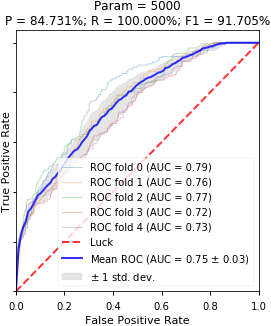
\includegraphics[width=1.4in]{ROC_RF} &
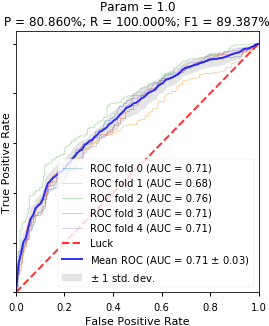
\includegraphics[width=1.4in]{ROC_NSVM} &
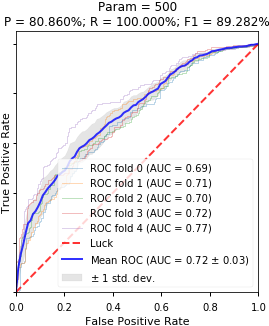
\includegraphics[width=1.4in]{ROC_GB} &
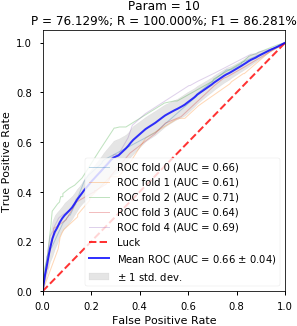
\includegraphics[width=1.53in]{ROC_GBLDA} 
\end{array}$
\end{center}
\caption{\label{ROC_init} ROC curves for the top four models (Left to right: Random Forests, Non-linear SVM and Gradient Boosting with PCA followed by Gradient Boosting with LDA)}
\end{figure}

\vspace{\baselineskip}
These results seem promising and Random Forests provide ideal performance on top predictions as we can also witness it on the ROC curve (c.f. Figure~\ref{ROC_init}) that is very steep and also presents the highest area under the curve. This means that even over all predictions, random forest outperforms the 3 other models. The model may require some extra tuning given its observable variability. 

\subsubsection{Improving Our Model Selection Process}
\paragraph{Problematic CV} Once we obtained such results we discovered that our estimate was incorrect. We tried to analyse how many days we could wait between training and predicting. In order to test this we needed to have a test set with dates that are non-overlapping with the training set. Even with 0 days past between the training and testing the classification metrics significantly dropped. The optimal model displayed above when tested on a test set made of 5 days yielded $P=51.25\%$. 

This proved the assumption that we formulated for the cross validation to be erroneous. It seems as if by training on same days as testing we overfit and overestimate performance metrics.	

\paragraph{Designing a New CV Strategy}
This pushed us to change the way we estimated the performance of our classifier. In order to have non-overlapping testing and training dates, we changed how we build each fold:
\begin{itemize}[noitemsep]
	\item From the full dataset, we derive the list of distinct dates and shuffle it. We end up with random indices $i$ for each date.
	\item To build a k-fold we assign day $i$ to the fold $i \text{ mod } k$ to homogeneously distribute dates over folds.
	\item Then we balance each training sets induced by each possible combination of $k-1$ folds.
\end{itemize}
With this strategy we ensure that we have balanced training sets as well as distinct dates between the training and testing sets. Figure~\ref{CV_comparison} illustrates the significant drop in estimated performance for the same model between the two CV techniques. 

\begin{figure}[h]
\begin{center}$
\begin{array}{cc}
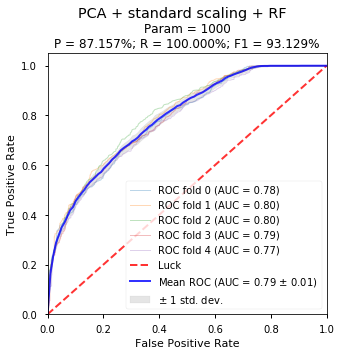
\includegraphics[width=2in]{old_cv} &
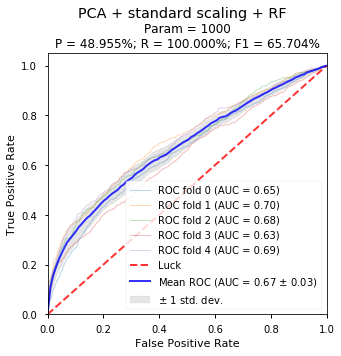
\includegraphics[width=2in]{new_cv} 
\end{array}$
\end{center}
\caption{\label{CV_comparison} Comparing old cross validation performance estimation (left) with the new one (right) on a Random Forest with 1000 trees with a PCA and standardised data}
\end{figure}


\paragraph{Graphical Performance Evaluation}
We would like to improve the previous model performance evaluation techniques and we followed multiple steps to do so.

So far we've been focusing on the top 20\% predictions in order to express the tradeoff between precision and recall on the 'sick' class. Nevertheless another technique would allow us to encapsulate such tradeoff. We could decide on different cutoff probabilities and look at the precision and recall for each. The cutoff probability is the value of the sick probability output by the model from which we start labeling samples as sick.

Also we let go of the ROC curve for Precision-Recall (PR) curves also called Calibration curves. These curves plot the precision against recall. Indeed it will be better in identifying good models in our imbalanced case (our test sets are left unbalanced). Suppose that we have a dataset with $500,000$ samples and only $100$ sick ones. and consider two algorithms:
\begin{itemize}[noitemsep,topsep=0pt]
	\item $\mathcal{A}_1$: 90 relevant out of the 100 identified
	\item $\mathcal{A}_2$: 90 relevant out of the 1000 identified
\end{itemize}
In our use case we would clearly prefer $\mathcal{A}_1$ over $\mathcal{A}_2$. Nevertheless if we compare PR and ROC curves we see that the first one distinguishes more easily the best algorithm:
\begin{itemize}
	\item ROC: 
		\begin{itemize}[noitemsep,topsep=0pt]
		\item $({TPR}_1,{FPR}_1)=(0.9,10/499,900)$
		\item $({TPR}_2,{FPR}_2)=(0.9,910/499,900)$
		\item Hence $|{FPR}_1-{FPR}_2|= 1.8\times 10^{-3}$
		\end{itemize}
	\item PR: 
		\begin{itemize}[noitemsep,topsep=0pt]
		\item $({P}_1,{R}_1)=(0.9,0.9)$
		\item $({P}_2,{R}_2)=(0.09,0.9)$
		\item Hence $|{P}_1-{P}_2|= 0.81$, wish shows that we distinguish models much more easily with such technique.
		\end{itemize}
\end{itemize}

We also had to derive a strategy to be able to cross validate a PR curve over different folds. Indeed, linear interpolation in the PR space yields an overly optimistic performance estimate~\cite{PRcurve} and because the probability thresholds used to build the curve for each fold may be different there isn't a trivial way to average curves. As suggested by past research~\cite{apples}, we will concatenate predictions and real targets of each test set and consider the PR curve constructed from these pooled predictions and true label datasets as our mean PR curve.

\paragraph{Metrics}
We also changed the metric that is monitored in order to determine the optimal model. As the business use of predictions entirely differs depending on the level of precision on the 'sick' class, we decided to use three precision levels $\{70\%,80\%,90\%\}$ that would be usable by business. We display on top of the PR curve the maximum recall that can be achieved for such precision. These metrics are computed on each fold and averaged overall. 

In order to determine the optimal model we will focus on the area under the PR curve. This will not exclusively evaluate the performance on top prediction but ensures that overall the model is optimal.

\subsubsection{Improved Research}
We performed the same kind of exploration but this time we also decided to try each model also without any dimensionality reduction algorithm (on standardised data). Indeed as we shall discuss it in the next subsection we realised that we may be losing information and hurting the performance of classifiers by blindly performing such compression.

\begin{table}[h]
\begin{center}
\begin{tabular}{c c c c c c c}
\hline
\textbf{Model} & \textbf{Dim. Red.} & \textbf{Parameter} & \textbf{AUC}& \textbf{R\textsubscript{70\%}(\%)} & \textbf{R\textsubscript{80\%}(\%)} & \textbf{R\textsubscript{90\%}(\%)} \\ 
\hline\hline
Gradient Boosting 	& - 		& 50 		& 0.528025 & 25.23 	& 18.51 & 10.48 \\
Random Forests 		& - 		& 5000		& 0.517642 & 24.06 	& 16.88 & 5.39\\
Non Linear SVM  	& - 		& 1	 		& 0.482226 & 18.55 	& 10.40 & 4.33\\
Linear SVM 			& PCA 	& 0.215443 	& 0.466997 & 17.57 	& 10.84 & 3.99\\
Logistic Regression & PCA 	& 0.003360 	& 0.472952 & 20.38 	& 11.68 & 3.91\\
Ridge Regression 	& PCA 	& 27.825594 	& 0.459569 & 18.93 	& 8.66 	& 3.15\\
\end{tabular}
\end{center}
\caption{\label{improved_results} Best results of the improved research ordered by decreasing R\textsubscript{90\%} (Maximum recall for 90\% precision)}
\end{table}

\begin{figure}[h]
\begin{center}$
\begin{array}{ccc}
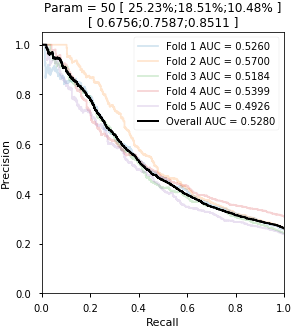
\includegraphics[width=1.8in]{PR_GB} &
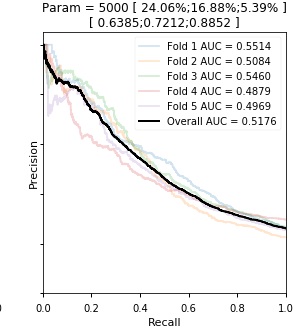
\includegraphics[width=1.8in]{PR_RF} &
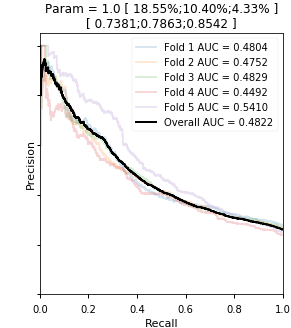
\includegraphics[width=1.8in]{PR_NSVM}
\end{array}$
\end{center}
\caption{\label{PR_curves} Precision Recall curves for the top 3 models obtained using the distinct date split. From left to right: Gradient Boosting, Random Forests, Non Linear SVM (always on standardised data). In the title of each graph we can observe the cutoff probability that yields the particular $(P,R)$ tuple.}
\end{figure}

We observe on Figure~\ref{PR_curves} that gradient boosting is more stable than the three other models as curves over different folds are grouped. The overall AUC is greater and we can see that the precision is high for more recall levels which also shows in R\textsubscript{90\%}, R\textsubscript{80\%} and R\textsubscript{70\%}. 

Given these results we focused on gradient boosting. The model is performing better without any dimensionality reduction as it requires fewer trees and is therefore simpler and quicker to train. 


\subsubsection{Understanding Classification}
\paragraph{No Dimensionality Reduction}
As advised by Felix Reisen from business intelligence, we wanted to check with the HFC support team if the most important features used by the model make sense. To perform such check we needed to look at the original features and not the components that are output by a dimensionality reduction technique. 

While trying out different ways to go from the most important components to the most important original features we tried to look at how the model performed without any dimensionality reduction. The overall better performance obtained pushed us to try to also explore this path in model coarse grain tuning and comparison. 

This strategy paid off as we can see that our top 3 models in previous subsection are not using any dimensionality reduction technique. 

\paragraph{Top 4 features}
Investigating the most important features of Gradient boosting gave us a good indication of the symptoms of failing CPEs. The most important feature was \texttt{OFFLINE\_PCT}, the percentage over Day\textsubscript{0} of offline hours. 


\begin{figure}[h]
\begin{center}$
\begin{array}{cc}
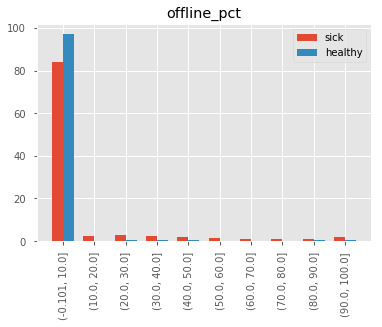
\includegraphics[width=2.55in]{most_imp_f_offline} &
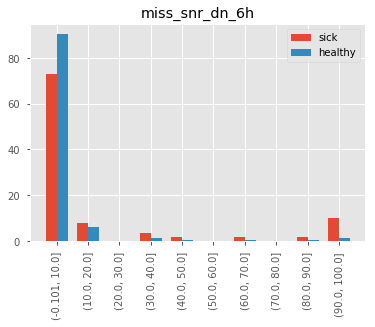
\includegraphics[width=2.5in]{most_imp_f_misssnr} \\
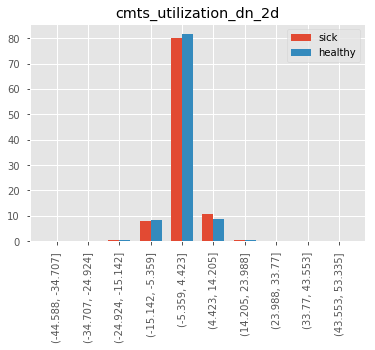
\includegraphics[width=2.5in]{most_imp_f_cmtsutil} &
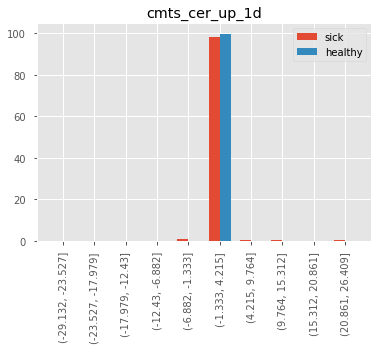
\includegraphics[width=2.5in]{most_imp_f_cmtscer}
\end{array}$
\end{center}
\caption{\label{most_important} 4 most important features distribution depending on the labels.}
\end{figure}


First of all, it is interesting as we also have a feature that gives the same percentage but over 6 hour windows but none are in the 4 most important features. That could indicate that customers do not have the same response time to call the technical help desk (THD) upon failure and therefore the percentage over 24 hours is more discriminative between classes. But also it gives us strong reasons to believe that a failing CPE is often time offline and this will influence the way me might handle predictions knowing that we may not be able to remotely service it. 

Also figure~\ref{most_important} confirms the usefulness of the CMTS level measurements as two such measurements are the 3rd and 4th most important features. The difference in distribution between labels couldn't be qualified as large, nevertheless we observe that for the \texttt{OFFLINE\_PCT} and \texttt{MISS\_SNR\_DN\_6H}, sick CPEs are less likely to be near zero.

According to Jonas, these indicators do make sense to identify internet problems and he expressed his desire to look at some CPEs predicted as failing to have more tangible results. We moved forward in our model tuning to be able to provide such examples. 

\subsection{Tuning Gradient Boosting}
Before we could present predictions to Jonas we had to fine-tune the model to make it optimal. We will present in this subsection how we fine-tuned the gradient boosting model, especially the new metric we decided to use, and the protocol we followed. Then we should look at the final model and visualise improvements added by the model relative to a baseline logistic regression.

\subsubsection{Protocol}
One should again consider that the proof of concept will not be used as a final model. Therefore an exhaustive grid search on each single parameters of the model may not be necessary. While we do want to display a well-adapted model, we are not interested in gaining 10\textsuperscript{th} of precision percentages as we only wish to prove that we can use the underlying patterns among failing CPEs to build a predictive model.

Also given the reduced time we had to tune the model and the diversity of hyper-parameters that can be adjusted, we had to limit the ones we would tune. Following popular practices~\cite{tuningGB}, we considered two steps:
\begin{itemize}
\item Tuning boosting parameters: focus on the number of estimators and the learning rate
\item Tuning tree based parameters: focus on the maximum depth of estimators and the minimum number of samples required to split a leaf node.
\end{itemize}
We are convinced that there is much greater work to be done on the data\footnote{As we should discuss it in chapter~\ref{chap:discussion}.} rather than the model itself, which is why we didn't spend too much time tuning the model. 

In order to report the performance of the model on the most recently collected dataset we present here the results based on a sample collected on the 27\textsuperscript{th} of June, time at which this section was draughted.

\subsubsection{Visualization}
At the time of this writing we realised that we forgot to test the model on unscaled data. Indeed due to its tree-based architecture, gradient boosting doesn't require scaling. Therefore we added the effect of this modification on our results but didn't use it in the model discussion as these tasks have been performed at an earlier time. 

\begin{table}[h]
\begin{center}
\begin{tabular}{c c c c }
\hline
\textbf{Model} & \textbf{R\textsubscript{70\%}} & \textbf{R\textsubscript{80\%}}& \textbf{R\textsubscript{90\%}}\\ 
\hline\hline
Linear Regression (scaled) & 24.8028\% & 15.6742\% & 4.7516\%  \\
Gradient Boosting (scaled) & 32.9851\% & 25.6919\% & \textbf{13.4116\%} \\
Gradient Boosting  &  \textbf{33.3239\%} & \textbf{26.2394\%} & 12.8978\%
\end{tabular}
\end{center}
\caption{\label{rec_models}Comparison of the performance (Maximum recall for a given precision) between our final model and the baseline.}
\end{table}

\begin{figure}[ht]
    \begin{center}
    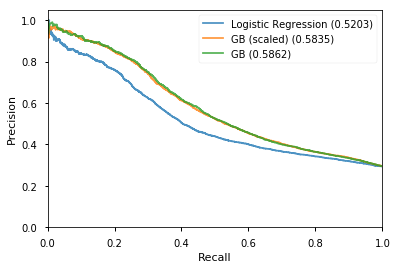
\includegraphics[width=0.6\linewidth]{images/model_comparison}
    \end{center}
	\caption{Calibration curves for final models against baseline}
    \label{model_comparison}
\end{figure}

On figure~\ref{model_comparison} we can observe that gradient boosting on unscaled data seems to be more stable at higher accuracy levels as the curve seems to be monotonous compared to the scaled version. This also illustrates the advantages of using PR curves to visually compare models: indeed if we were to look only at R\textsubscript{90\%} in table~\ref{rec_models}, we could believe the scaled version to perform better. We would like to note that we haven't displayed on the plot for visibility concerns the PR curve of each fold which means that one should be careful when comparing curves that could in reality describe variable models. 

\subsection{Model Discussion}
Once we had our final model, we were ready to analyse predictions. We first started by trying to predict a given day and go the same day to the HFC support team to review these predictions and see how they assess the quality of the model. Then we tried to perform again an analysis of how the number of days between training and predicting would affect the performance of the model. Finally, we briefly looked at one of our hypotheses regarding why standard cross validation caused a performance overestimation.

\subsubsection{Model Output Check}
On the 11\textsuperscript{th} of June, we trained the model on the dataset that we had collected up to this point and predicted potential failures. Once the model is tuned, we obtain 3 thresholds which are the probability thresholds that should help us reach particular $(P,R)$ pairs. 

At first we tried to use the highest threshold and found no MAC with a sick probability satisfying this threshold. Therefore we used the second threshold and one MAC was predicted as failing at this particular 'confidence level'. To leverage as much as possible the time that the HFC support team allocated to review our predictions with us we decided to also predict on all days that were not in the training set\footnote{It is important to remember that the training  set can only be constructed up to 8 days prior to the current date as explained in section~\ref{subsec:collecting}.}. That allowed us to generate more predictions and therefore come to the meeting with more material to analyse.

\begin{table}[h]
\begin{center}
\begin{tabular}{c c c p{90mm}}
\hline
\textbf{MAC} & \textbf{$p_\text{sick}$} & \textbf{Day\textsubscript{1}} & \textbf{Comment} \\ 
\hline\hline
\texttt{54:67:51:F4:0E:59} & 0.778949 & 10/06 & One HFC interface is continuously resetting, during this period the customer has no connection. Probably a hardware modem issue. \textbf{True positive}\\
\hline
\texttt{AC:22:05:9A:C2:21} & 0.892083 & 09/06 & Went offline for an extended amount of time. Nevertheless the many missing values could indicate a data polling issue. \textbf{False positive} but presents irregularities\\
\hline
\texttt{C4:27:95:17:77:A7} & 0.821313 & 07/06 & Lots of packets dropped on one of the channels, this can result for the customer in performance issues (service degradations). It is most probably a cabling problem that can be solved by the customer thanks to a replacement cable. \textbf{True positive}\\
\hline
\texttt{90:5C:44:BF:63:96} & 0.783860 & 06/06 &  We can see that levels were down for an extended period of time and went back up, which should indicate a technician intervention. We couldn't find it but given the similarities we can conclude that this is a \textbf{true positive}.\\
\end{tabular}
\end{center}
\caption{\label{checks} Four CPEs predicted as failing and review with the HFC support team}
\end{table}

As displayed in table~\ref{checks}, out of four predictions reviewed, three were true positives. Also Jonas expressed great satisfaction regarding the model as even the False positive presented some issues that could have thrown off the model. This reality check was necessary to ensure that the POC was pointing in the right direction as, up to this point, we based all our performance on metrics that rely on a ground truth that can be criticised. 

In order to review these predictions, the HFC team uses a tool based on SAA to display different health measurements of CPEs. In chapter~\ref{chap:discussion} we will discuss a specificity of this tool, as experts use value thresholds in order to track some performance indicators which could be leveraged by a future project.

\subsubsection{Time Gap Influence}
We repeated the analysis that we conducted earlier and made us realise our mistake using a standard cross validation. Because so far we can only train up to 8 days before the current date we looked at how the time between training and predicting influenced performances.

In order to estimate properly performances, we used all our available dates to cross validate our curves. We created multiple training set and testing set pairs with the correct time gap between them to generate our metrics. 

\begin{figure}[ht]
    \begin{center}
    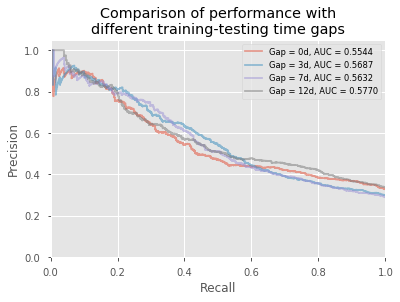
\includegraphics[scale=0.7]{time_gap}
    \end{center}
    \caption{Influence of time between the model is trained and used to generate prediction}
    \label{time_gap}
\end{figure}

Figure~\ref{time_gap} shows that we cannot identify a significant influence of time. Should there be an influence we would have expected to see the decreasing performance as time past. This supports the fact that the model can be used during an extended period of time without the need to be retrained every single day. 

\subsubsection{Same Weekday Training/Testing}
As stated earlier, our intuition regarding why our initial cross validation failed miserably was that training on dates that are also in the testing set may result in overfitting. We wondered whether we were not overfitting particular weekdays. To answer this question we created from the dataset, 7 subsets made only of identical weekdays. Then we generated our cross validated PR curves on each dataset to see if we would observe an increase of performance. By nature, this should not be conclusive as gradient boosted trees can use the \texttt{WEEK\_DAY} feature that we created to create sub-models for each day. 

\begin{figure}[h]
\begin{center}$
\begin{array}{c}
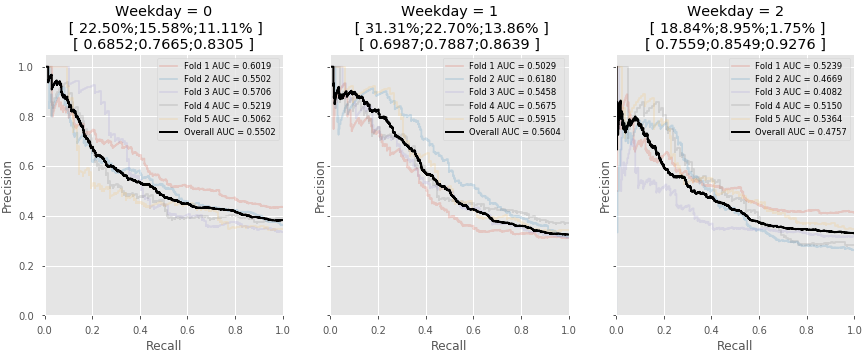
\includegraphics[scale=0.4]{weekdays_1} \\
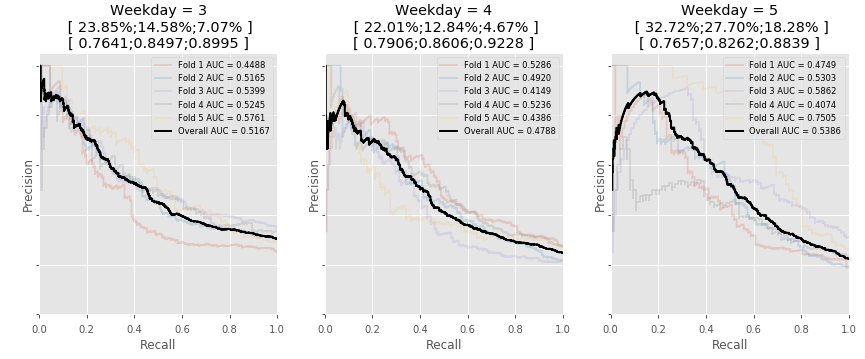
\includegraphics[scale=0.4]{weekdays_2} \\
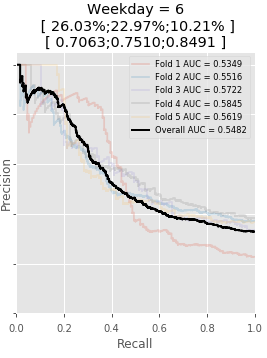
\includegraphics[scale=0.4]{weekdays_3} 
\end{array}$
\end{center}
\caption{\label{weekdays} Cross validated calibration curves for weekday subsets}
\end{figure}

Indeed, we can observe that the resulting performances (cf. figure~\ref{weekdays}) are not increased therefore ruling out our intuition that particular weekdays are overfitted. An interesting observation is the relative instability of the models on weekend days, compared to other days, that could confirm our intuition regarding the potential benefit of discarding weekend days from our analysis (cf. section~\ref{subsec:influence}). 

\vspace{\baselineskip}
We have successfully built a proof of concept that shows evidence of pattern in CPE failures that could be leveraged by UPC. Our intermediary analysis allowed us to have a better understanding of the data and also to spot some initial problems that would need to be mitigated in the future. Our attempt at clustering wasn’t conclusive but highlighted the power of some dimensionality reduction techniques and pushed for the need to have lower-dimensional space. Finally, the model exploration process presented iterative refinement of our goals and methods that will add great value to further research. 